\section{摩擦力}
\subsection{定义}
阻碍物体\CJKunderwave{相对运动}(或者\CJKunderwave{相对运动趋势})的力叫做摩擦力.
\subsection{方向}
摩擦力存在于相互接触的两个物体间,则\CJKunderwave{受力物体所受摩擦力}的方向与\CJKunderwave{受力物体相对于施力物体的运动(或相对运动趋势)}的方向相反.

同学们注意,相对运动这点比较容易看出来,但是相对运动的趋势则用肉眼不能看出来,解决的方法是\CJKunderwave{假设法},即:假设没有摩擦则看物体将向哪个方向运动,则此运动方向就是相对运动趋势的方向.相对运动的趋势本质上是微观上原子之间相对位置发生了变化,但是没有宏观上的运动.

\subsection{摩擦力的分类}
\subsubsection{静摩擦力}
两个相互接触的物体,当其接触表面之间有相对运动的趋势,但尚保持相对静止时,彼此作用着阻碍相对滑动的阻力,这种阻力称为静滑动摩擦力,简称为静摩擦力.静摩擦力产生的条件为:
\begin{enumerate}
  \item 相互接触,且接触面粗糙
  \item 有弹力(或者形变)
  \item 有相对运动的趋势
\end{enumerate}

静摩擦力的大小是一个范围,它会根据外界的受力情况而自动作出调整.当外力超过一定的限度时,物体和物体之间将会发生相对滑动,能够保持物体之间相对静止的最大的静摩擦力叫做最大静摩擦力,用符号$f_{max}$  表示.用公式表达就是
\begin{equation}
  0\leqslant f\leqslant f_{max}
  \label{eq:jingmoca}
\end{equation}

\subsubsection{滑动摩擦力}
当一物体在另一物体表面上滑动时,在两物体接触面上产生的阻碍它们之间相对滑动的力叫做滑动摩擦力.滑动摩擦力产生的条件为:
\begin{enumerate}
  \item 相互接触,且接触面粗糙
  \item 有弹力(或者形变)
  \item 有相对运动
\end{enumerate}

滑动摩擦力的大小,由库仑摩擦定律来确定,即下式
\begin{equation}
  f=\mu F_N
  \label{eq:dongmoca}
\end{equation}

在\eqref{eq:dongmoca} 式中,$\mu$叫做动摩擦因数,取决于相互接触的两个物体在粗糙程度和材料等因素.$F_N$ 是二物体接触面的正压力,$f$ 是滑动摩擦力.由\eqref{eq:dongmoca}式容易得到\CJKunderwave{滑动摩擦力与接触面积无关}.

\subsubsection{滚动摩擦力}
一物体在另一物体表面做无滑动的滚动或有滚动的趋势时,由于物体在接触部分受压发生形变而产生的对滚动的阻碍作用,叫滚动摩擦.它的实质是静摩擦力.由于在高中阶段暂未涉及滚动摩擦力,这里提出来仅作为知识上的完备,不作深入讨论.

\subsection{例题分析}

\begin{selection}
1.如<:
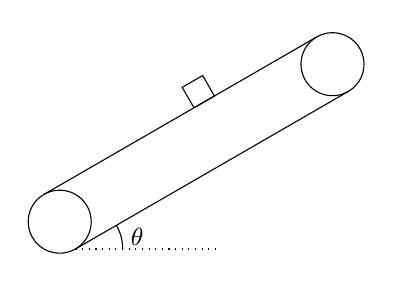
\begin{tikzpicture}
  \draw [dotted] (0.2,0.053589838)--(2,0.053589838); 
  \draw (0,0.4) circle [radius=0.4cm] ;
  \draw[rotate around={30:(0,0.4)}] (4,0.4) circle [radius=0.4cm] ;
  \draw[rotate around={30:(0.2,0.053589838)}] (0.2,0.053589838)--(4.2,0.053589838); 
  \draw[rotate around={30:(-0.2,0.7464)}] (-0.2,0.7464)--(3.8,0.7464); 
  \draw[rotate around={30:(-0.2,0.7464)}] (2,0.7464) rectangle (2.3,1.0464); 
  \draw (0.8,0.053589838) arc (0:30:0.6);
  \draw [rotate around={15:(0.2,0.053589838)}] (0.8,0.053589838) node [anchor=west]{\small $\theta$};
\end{tikzpicture}
:>所示,为倾斜的皮带传送装置.关于传送带上的物体所受的摩擦力,下列说法正确的是
A.若传送带静止,物体也静止,则物体受到沿传送带向上的摩擦力
B.若传送带静止,物体也静止,则物体受到沿传送带向下的摩擦力
C.若传送带顺时针匀速转动,物体随传送带一起向做匀速运动,则物体受到沿传送带向上的静摩擦力
D.若传送带顺时针匀速转动,物体随传送带一起向做匀速运动,则物体受到沿传送带向上的滑动摩擦力
  
a.AC

e.物体静止在静止的传送带上时,或物体随传送带一起向上匀速运动的过程中,都具沿传送带下滑的趋势,这个趋可以假设传送带光滑然后物体一定在重力作用下向下滑动判断出来,所以物体均受到沿传送带向上的静摩擦力作用.

\end{selection}

\begin{calculate}
  2.如<:
  \begin{tikzpicture}
   \draw (-1,0) rectangle (1,1); 
   \draw (0,0.5) node {B};
   \draw (-0.5,1) rectangle (0.5,1.5);
   \draw (0,1.25) node {A};
   \draw [->](1,0.5) -- (2,0.5) node [anchor = south] {F};
   \draw [pattern=north west lines] (-1.5,-0.2)--(-1.5,0)--(2.5,0)--(2.5,-0.2);
  \end{tikzpicture}
  :>所示,物体$A$ ,$B$ 在外力作用下共同做匀速运动,$A$ 是否受到摩擦力?

  a.不受摩擦力

  e.$A$ 物体保持静止,所以受力是平衡的,假设$A$ 受到摩擦力,但是在水平方向找不到一个力与此力平衡的力,所以假设错误,因此$A$ 不受摩擦力.

  3.质量为$2kg$ 的物体静止在水平地面上,如<:
  \begin{tikzpicture}
    \draw (0,0) rectangle (1.5,1);
    \draw [->] (2.5,0.5) node [anchor=west]{\small $F$} -- (1.5,0.5);
   \draw [pattern=north west lines] (-0.5,-0.2)--(-0.5,0)--(3,0)--(3,-0.2);
  \end{tikzpicture}
  :>所示,物体与地面间的动摩擦因数为$0.5$ ,最大静摩擦力与滑动摩擦力视为相等,给物体一水平推力$F$.(取$g=10m/s^2$)

  a.(1) $5N$ \qquad (2) $10N$ \qquad (3) $10N$

  e.在地面上,由竖直方向受力平衡得$F_N=mg$ ,则滑动摩擦力由\eqref{eq:dongmoca} 式得
  $$f=\mu F_N=0.5\times 2\times 10N=10N$$
  题中认为最大静摩擦力等于滑动摩擦力,所以$f_{max}=10N$
  \newline
  (1)当推力$F=5N$ 时,$F<f_{max}$ ,则物体保持静止,由二力平衡知,地面对物体的静摩擦力大小为
  $$F_{\mbox{\tiny 静}}=F=5N$$
  (2)当推力$F=12N$时,$F>f_{max}$,物体滑动.则地面对物体的滑动摩擦力大小为
  $$F_{\mbox{\tiny 滑}}=\mu F_N=\mu mg=10N$$
  (3)物体运动过程中突然把推力去掉,地面对物体的摩擦力为滑动摩擦力,其大小同(2)中计算得
  $$F_{\mbox{\tiny 滑}}=\mu F_N=\mu mg=10N$$

\end{calculate}
